%-------------------------------------------------------------------------------
\chapter{Constraints of surface contacts}
\label{app.surface_contacts}
\acresetall
%-------------------------------------------------------------------------------


%%%%%%%%%%%%%%%%%%%%%%%%%%%%%%%%%%%%%%%%%%%%%%%%%%%%%%%%%%%%%%%%%%%%%%%%%%%%%%%%
%%%%%%%%%%%%%%%%%%%%%%%%%%%%%%%%%%%%%%%%%%%%%%%%%%%%%%%%%%%%%%%%%%%%%%%%%%%%%%%%
%%%%%%%%%%%%%%%%%%%%%%%%%%%%%%%%%%%%%%%%%%%%%%%%%%%%%%%%%%%%%%%%%%%%%%%%%%%%%%%%
\section{Rectangular foot contact}\label{sec.rectangular_foot}

Foot contact with the ground is the most common type of contact realized by
humanoid robots. A foot typically consists of one or two, if the robot has toes,
rigid bodies with flat soles. Contact of a sole with the ground is often
characterized by 3-dimensional contact forces applied at $N$ vertices of the
support polygon as shown in \cref{fig.friction_foot_vertex}
\cite{Kuindersma2014icra, Abe2007siggraph, Ott2011humanoids, Hauser2008ijrr}.
In this case, the interaction with the support surface is described by $3N$
force variables, which are redundant, since the number of degrees of freedom of
a rigid body does not exceed $6$. The redundancy leads to excessive number of
constraints and variables, which have negative impact on computational
performance and may cause numerical problems in solvers. For this reason, here
we consider a more concise representation of interaction between a rectangular
sole and support by a single wrench. The wrench is computed with respect to the
origin of a frame fixed to the middle of the sole as illustrated in
\cref{fig.friction_foot_center}. All variables used below in the derivations
are expressed in the said frame, therefore, appropriate transformations must be
performed to switch to the global frame.


\begin{figure}[ht]
    \begin{minipage}[t]{0.48\textwidth}
        \centering{%
        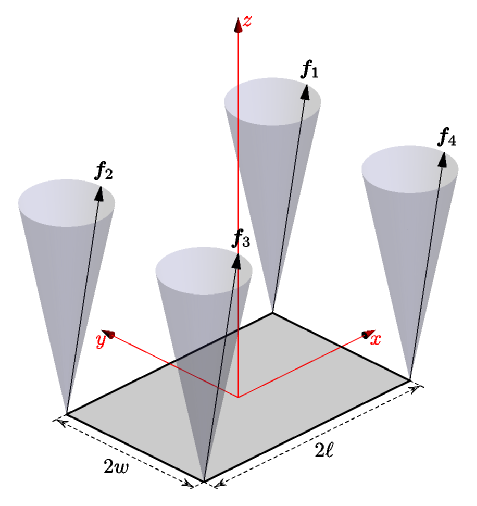
\includegraphics{friction_foot_vertex.eps}}
        \subcaption{
            Contact forces are comprised of four 3-dimensional force vectors
            ($\V{f}_1, ..., \V{f}_4$) applied at the corners of the support
            area.
        }
        \label{fig.friction_foot_vertex}
    \end{minipage}
    \hfill
    \begin{minipage}[t]{0.48\textwidth}
        \centering{%
        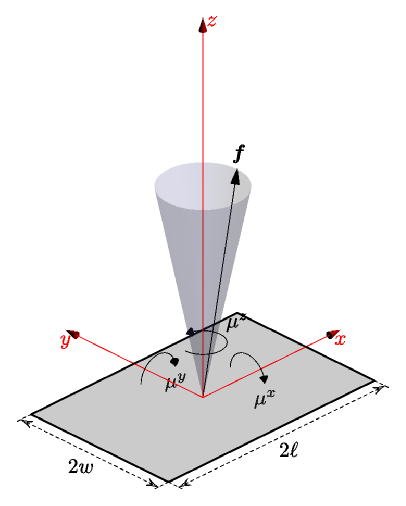
\includegraphics{friction_foot_center.eps}}
        \subcaption{
            Contact forces are comprised of a single 6-dimensional wrench
            ($\V{f}, \moment$) applied at the center of the support area.
        }
        \label{fig.friction_foot_center}
    \end{minipage}
    \caption[Representation of the foot contact forces.]{
        Representation of foot contact forces. Grey rectangles are rectangular
        foot support areas of length $2\ell$ and width $2w$, cones are
        Coulomb's friction constraints.
    }
    \label{fig.friction_foot}
\end{figure}


Let us integrate over the support area $\SET{S}$ to obtain the total contact
force~\cite{Howe1996ijrr}
%
\begin{subequations}
\begin{align}
    \begin{bmatrix}
        f^x\\
        f^y\\
    \end{bmatrix}
    &=
    \int_{\SET{S}}
    {
        \tilde{\friction}(x,y)
        \V{v}(x,y)
        \,
        df^z(x,y)
    },\\
    f^z
    &=
    \int_{\SET{S}}
    {
        \,
        df^z(x,y)
    }\label{eq.force_z_integral},
\end{align}
\end{subequations}
%
where $\V{v}(x,y)$ is a unit vector of the tangential contact force at a given
point, $\tilde{\friction}(x,y) \in [0, \friction]$ relates the norms of the
tangential and the normal forces, and integration is performed with respect to
$f^z(x,y) \ge 0$ to account for potential discontinuities in pressure
distribution. Norm of the tangential contact force reaches maximal value when
tangential forces at each point of $\SET{S}$ are collinear $\V{v}(x,y) = \V{v}$
and parameter $\tilde{\friction}(x,y)$ is equal to the friction coefficient
$\friction$, hence
%
\begin{equation}
    \V{f}^{xy}_{\MT{max}}
    =
    \int_{\SET{S}}
    {
        \friction
        \V{v}
        \,
        df^z(x,y)
    }
    =
    \friction
    f^z
    \V{v}.
\end{equation}
%
This implies that the total tangential contact force is limited to the friction
cone, which can be linearized as described in \cref{sec.contact_constraints}.


We continue by obtaining the total contact moment
%
\begin{subequations}
\begin{align}
    \begin{bmatrix}
        \momentC^x\\
        \momentC^y\\
    \end{bmatrix}
    &=
    \int_{\SET{S}}
    {
        \begin{bmatrix}
            y\\
            -x
        \end{bmatrix}
        \,
        df^z(x,y)
    }, \label{eq.moment_xy_integral}\\
    \momentC^z
    &=
    \int_{\SET{S}}
    {
        \tilde{\friction}(x,y)
        \begin{bmatrix}
            -y & x
        \end{bmatrix}
        \V{v}(x,y)
        \,
        df^z(x,y)
    } \label{eq.moment_z_integral}.
\end{align}
\end{subequations}
%

First we focus on Equation~\cref{eq.moment_xy_integral}. It is straightforward
that the moments about the $x$ and $y$ axes take their maximal values, when the
normal contact force is applied at the respective edges of the support area,
\IE, when $x = \pm \ell$ or $y = \pm w$, consequently,
%
\begin{equation}\label{eq.moment_xy_bounds}
    -
    \begin{bmatrix}
        w\\
        \ell\\
    \end{bmatrix}
    f^z
    \le
    \begin{bmatrix}
        \momentC^x\\
        \momentC^y\\
    \end{bmatrix}
    \le
    \begin{bmatrix}
        w\\
        \ell\\
    \end{bmatrix}
    f^z.
\end{equation}
%
Significance of these inequalities becomes clear after division of
\cref{eq.moment_xy_integral} by \cref{eq.force_z_integral}:
%
\begin{equation}
    \frac{1}{f^z}
    \begin{bmatrix}
        \momentC^x\\
        \momentC^y\\
    \end{bmatrix}
    =
    \frac{
        \int_{\SET{S}}
        {
            \begin{bmatrix}
                y\\
                -x
            \end{bmatrix}
            \,
            df^z(x,y)
        }
    }
    {
        \int_{\SET{S}}
        {
            \,
            df^z(x,y)
        }
    }
    =
    \begin{bmatrix}
        \copC^y\\
        -\copC^x
    \end{bmatrix},
\end{equation}
%
where $\cop = (\copC^x, \copC^y) = (-\momentC^y, \momentC^x) / \forceC^z$ is
position of \ac{CoP} of the contact pressure field. Thus, constraints
\cref{eq.moment_xy_bounds} imply that $\cop \in \SET{S}$, but they also remain
valid when \ac{CoP} is not defined, \IE, when $f^z = 0$. Furthermore,
\cref{eq.moment_xy_bounds} can be generalized to arbitrary convex polygonal
support areas, when the constraints take the following form \cite{Nagasaka2012}
%
\begin{equation}
    a \momentC^x + b \momentC^y \le c f^z,
\end{equation}
%
where $a,b,c$ are parameters of a line defining a face of the support polygon.


Analysis of Equation~\cref{eq.moment_z_integral} is more intricate. In order to
illustrate this let us assume that $\tilde{\friction}(x,y) = \tilde{\friction}$
and $\V{v}(x,y) = \V{v}$. Then
%
\begin{equation}
    \momentC^z
    =
    \int_{\SET{S}}
    {
        \tilde{\friction}
        \begin{bmatrix}
            -y & x
        \end{bmatrix}
        \V{v}
        \,
        df^z(x,y)
    }
    =
    \tilde{\friction}
    \T{\V{v}}
    \int_{\SET{S}}
    {
        \begin{bmatrix}
            -y \\
            x
        \end{bmatrix}
        \,
        df^z(x,y)
    }
    =
    -
    \tilde{\friction}
    \T{\V{v}}
    \begin{bmatrix}
        \momentC^x \\
        \momentC^y
    \end{bmatrix},
\end{equation}
%
which can be multiplied by $\forceC^z$ to obtain
%
\begin{equation}
    \momentC^z \forceC^z
    =
    -
    \forceC^x
    \momentC^x
    -
    \forceC^y
    \momentC^y.
\end{equation}
%
Thus, under the assumption that all tangential forces are collinear, the moment
about the $z$ axis is nonlinearly determined by other components of the wrench.
In fact, under this assumption the total contact moment is computed by the
cross product of the \ac{CoP} position and the total contact force. In general,
however, we cannot make such assumption and should avoid nonlinear constraints.
Instead, we compute the absolute minimum and maximum of $\momentC^z$, which are
achieved when the origin of the frame is the center of rotation
%
\begin{equation}
    \V{v}
    =
    \pm
    \frac{1}{\sqrt{x^2 + y^2}}
    \begin{bmatrix}
        -y \\
        x
    \end{bmatrix}
\end{equation}
%
and $\tilde{\friction}(x,y) = \friction$. Hence, the bounds on $\momentC^z$ are
%
\begin{equation}
    \ubar{\momentC}^z
    =
    -
    \friction
    \int_{\SET{S}}
    {
        \sqrt{x^2 + y^2}
        \,
        df^z(x,y)
    },
    \quad
    \bar{\momentC}^z
    =
    \friction
    \int_{\SET{S}}
    {
        \sqrt{x^2 + y^2}
        \,
        df^z(x,y)
    }.
\end{equation}
%
They reach the minimal (maximal) values when the normal contact force is
concentrated in the corners of $\V{S}$ with coordinates $(\pm \ell, \pm w)$, so
that
%
\begin{equation}\label{eq.moment_z_bounds}
    \ubar{\momentC}^z
    =
    -
    \friction
    \sqrt{\ell^2 + w^2}
    f^z,
    \quad
    \bar{\momentC}^z
    =
    \friction
    \sqrt{\ell^2 + w^2}
    f^z.
\end{equation}
%
Note that these bounds must be tighter if any of the following holds true:
\begin{itemize}
    \item $\tilde{\friction}(x,y) < \friction$;
    \item the center of rotation does not coincide with the center of the foot;
    \item the pressure is not concentrated in the corners of $\SET{S}$.
\end{itemize}
However, constraints \cref{eq.moment_z_bounds} have found their application in
contact modeling due to their simplicity and linearity \cite{Fujimoto1996icra,
Bouchard2015gic}. Constraints of a similar form
%
\begin{equation}
    -\tilde{\friction} \forceC^z \le \momentC^z \le \tilde{\friction} \forceC^z,
\end{equation}
where $\tilde{\friction}$ is a certain torsional friction coefficient, are also applied
\cite{Mansour2013iros, Nagasaka2012}, especially in the works using the so
called \tn{soft finger} contact model for grasping
\cite[Chapter~5]{Murray1994mathematical}. Other approaches to limitation
of $\momentC^z$ include
%
\begin{itemize}
    \item Complete omission of the bounds \cite{Stephens2010iros,
        Audren2014iros, Henze2014iros, Herzog2015auro}. This, however, is more
        dangerous than imposing \cref{eq.moment_z_bounds}.

    \item Construction of more elaborate bounds depending on $\moment^{xy}$ and
        $\force^{xy}$ \cite{Caron2015icra}. Unfortunately, obscurity of the
        derivations makes it difficult to analyze implications of these
        constraints.

    \item Derivation of the bounds based on certain assumptions about
        distribution of the contact pressure \cite{Zhu2006iros,
        Zhou2013robotica}.

    \item Use nonlinear bounds with some additional assumptions
        \cite[Chapter~5]{Yamane2004figures}.
\end{itemize}
%


We draw two conclusions from the present discussion: the total tangential
contact force is subject to Coulomb's friction constraints in the same way as
in the case of a point contact; the contact moments can and should be bounded
using \cref{eq.moment_xy_bounds} and \cref{eq.moment_z_bounds}, which are
summarized as
%
\begin{equation}
    \forceC^n
    \underbrace{
        \begin{bmatrix}
            -w\\
            -\ell\\
            -\sqrt{\ell^2 + w^2}
        \end{bmatrix}
    }_{\ubar{\moment}}
    \le
    \moment
    \le
    \forceC^n
    \underbrace{
        \begin{bmatrix}
            w\\
            \ell\\
            \sqrt{\ell^2 + w^2}
        \end{bmatrix}
    }_{\bar{\moment}}.
\end{equation}


%%%%%%%%%%%%%%%%%%%%%%%%%%%%%%%%%%%%%%%%%%%%%%%%%%%%%%%%%%%%%%%%%%%%%%%%%%%%%%%%
%%%%%%%%%%%%%%%%%%%%%%%%%%%%%%%%%%%%%%%%%%%%%%%%%%%%%%%%%%%%%%%%%%%%%%%%%%%%%%%%
%%%%%%%%%%%%%%%%%%%%%%%%%%%%%%%%%%%%%%%%%%%%%%%%%%%%%%%%%%%%%%%%%%%%%%%%%%%%%%%%
\section{General surface contacts}\label{sec.surface_contacts}

Surface contacts are not necessarily rectangular: multiple contacts with the
same surface may lead to a support area of a rather complex shape. For example,
when the robot walks on a flat ground, it may have two foot contacts with the
ground at the same time. The support area in this case is the convex hull
$\SET{S}(\contact_1^{xy},\contact_2^{xy})$ of two rectangular feet with
positions $\contact_1^{xy}$ and $\contact_2^{xy}$ (see
\cref{fig.support_area_ctr}). Walking with coplanar contacts is so common that
some approximate models were specifically designed for this task, in
particular, the point-mass models considered in
\cref{sec.point_mass_planar,sec.point_mass_nonplanar}. For this reason, we
discuss general surface contacts in more detail here.


\begin{figure}[ht]
    \centering{%
    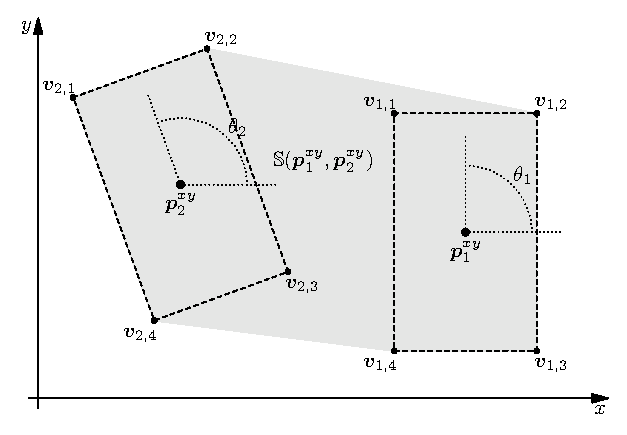
\includegraphics{support_area_ctr.eps}}
    \caption[Constraints on position of the Center of Pressure.]{
        Grey area represents support area $\SET{S}(\contact_1^{xy},
        \contact_2^{xy})$ of two rectangular foot contacts.
    }
    \label{fig.support_area_ctr}
\end{figure}


From the preceding section it is clear that bounding of the tangential contact
forces is easy (see also \cref{sec.point_mass_nonlinear}). At the same time,
derivation of the bounds on the contact moment about the $z$ axis is nontrivial
even in the case of a simple rectangular shape. Therefore, we entirely focus on
the constraints on moments about the $x$ and $y$ axes. Provided that the normal
force is nonzero, these constraints are equivalent to constraints on the
\ac{CoP} position: $\cop \in \SET{S}(\contact_1^{xy}, \contact_2^{xy})$. One
way to express these constraints is to find faces of the support polygon and
force $\cop$ to stay on their inner side with inequality constraints. These
inequalities, however, are difficult to parametrize with respect to positions
$(\contact_1^{xy}, \contact_2^{xy})$ and orientations of the feet $(\theta_1,
\theta_2)$. Therefore, we consider constraints on the \ac{CoP} using a
different approach: we exploit the fact that as long as the \ac{CoP} lies
within the support area it is a convex combination of vertices $\V{v}_{i,j} \in
\RR^2$ with $i \in \{1,2\}$ and $j \in \{1,2,3,4\}$ of the rectangular foot
contacts shown in \cref{fig.support_area_ctr}.


Since the \ac{CoP} is a convex combination of vertices $\V{v}_{i,j}$, we express
it as
%
\begin{equation}
    \cop
    =
    \sum_{j=1}^{4}
    \left.
        \sum_{i=1}^{2}
            \eta_{i,j} \V{v}_{i,j}
    \right.
    ,
    \quad
    \sum_{j=1}^{4}
    \left.
        \sum_{i=1}^{2}
            \eta_{i,j}
    \right.
    =
    1,
    \quad
    \eta_{i,j}
    \ge
    0
    .
\end{equation}
%
Let us denote positions of vertices of a given foot expressed in a frame fixed
to its center as $\V{v}_{\{1,2,3,4\}}$. Then $\V{v}_{i,j} = \hatM[i]{R}\V{v}_j
+ \contact_i^{xy}$, where $\hatM[i]{R}$ is a rotation matrix depending on
$\theta_i$. Hence,
%
\begin{equation}
    \begin{aligned}
        &
        \cop
        =
        \sum_{j=1}^{4}
        \left(
            \left(
            \sum_{i=1}^{2}
                \eta_{i,j} \hatM[i]{R}
            \right)
            \V{v}_{j}
        \right)
        +
        \left(
        \sum_{j=1}^{4}
            \eta_{1,j}
        \right)
        \hatM[1]{R}
        \contact_1^{xy}
        +
        \left(
        \sum_{j=1}^{4}
            \eta_{2,j}
        \right)
        \hatM[2]{R}
        \contact_2^{xy}
        ,
        \\
        &
        \sum_{j=1}^{4}
        \left.
            \sum_{i=1}^{2}
                \eta_{i,j}
        \right.
        =
        1,
        \quad
        \eta_{i,j}
        \ge
        0
        .
    \end{aligned}
\end{equation}
%
Since $\V{v}_{j}$ are constant, the \ac{CoP} position is determined by
coefficients $\eta_{i,j}$, foot positions $\contact_i^{xy}$, and foot
orientations $\theta_i$. This relation is linear in several cases:
%
\begin{itemize}
    \item Positions and orientations of the feet are fixed. Then variables
        $\eta_{i,j}$ determine position of the \ac{CoP}.

    \item Orientations of the feet are fixed and distribution of the pressure
        between the feet is known, \IE,
        %
        \begin{equation}
            \sum_{j=1}^{4}
                \eta_{1,j}
            =
            \MT{const}
            ,
            \quad
            \sum_{j=1}^{4}
                \eta_{2,j}
            =
            \MT{const}.
        \end{equation}
        %
        In this case positions of the feet and, to some extent, position of the
        \ac{CoP} can vary.

    \item There is only one contact with the surface and orientation of the
        foot is fixed. Then, in addition to position of the \ac{CoP} within the
        foot, the position of the foot can vary. This allows to anticipate
        walking motions without predetermined contact positions
        \cite{Herdt2010auro, Sherikov2014humanoids}.
\end{itemize}
%


Though nonlinear \ac{MPC} allows to handle nonlinear constraints on the
\ac{CoP} position \cite{Naveau2016ral}, in practice it is common to employ
approximations, for example,
%
\begin{itemize}
    \item Support area in a double support can be approximated using support
        area of a single support, which is translated and oriented
        appropriately as demonstrated in \cref{fig.ds_approximation}
        \cite{Dimitrov2011icra}, \cite[Chapter~3]{Sherikov2012master}.

        %
        \begin{figure}[ht]
            \centering{%
            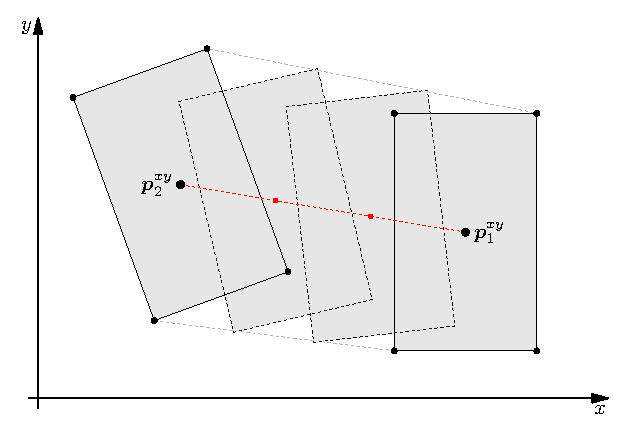
\includegraphics{ds_approximation.eps}}
            \caption[Approximation of the support area in a double support.]{
                Approximation of the support area in a double support with
                support area of a single support.
            }
            \label{fig.ds_approximation}
        \end{figure}
        %

    \item The support area does not depend on foot orientations in the case of
        point or round feet. Therefore, we can constrain the \ac{CoP} positions
        to conservative round support areas as illustrated in
        \cref{fig.support_rotations} \cite{Lafaye2014humanoids}. This
        guarantees that the \ac{CoP} position always stays within the real
        support area. Alternatively, orientations of the feet can be
        precomputed using a dedicated \ac{MPC} scheme as proposed in
        \cite[Chapter~2]{Herdt2012thesis},

        %
        \begin{figure}[ht]
            \centering{%
            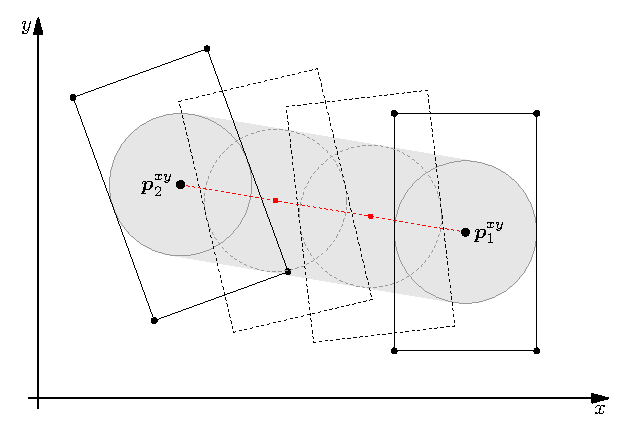
\includegraphics{support_rotations.eps}}
            \caption[Support area, which is independent of foot orientations.]{
                Grey area demonstrates support area, which is independent of
                foot orientations.
            }
            \label{fig.support_rotations}
        \end{figure}
        %
\end{itemize}
